%! Tex program = xelatex
\documentclass[UTF8]{article}
\usepackage{indentfirst}
\usepackage{graphicx} 
\usepackage{amsmath}  
\usepackage{float}   
\usepackage{listings}

\title{Discrete Mathematics}
\author{Zhengren Wang 2019081308021}
\date{06/02/2020 Tue}
\begin{document}
\maketitle 

\part{10.6}
\begin{description}
    \item[3]Find the length of a shortest path between $a$ and $z$ in the given weighted graph. \\
        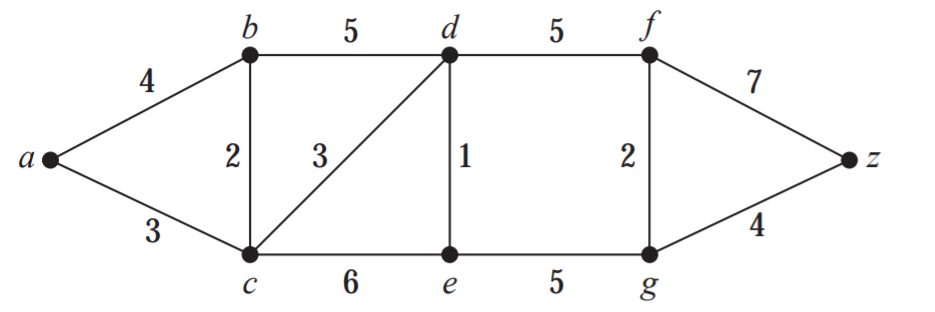
\includegraphics[scale=0.3]{../imgs/10_6_3.png}\\\\
        the length of $a,c,d,e,g,z$ is 16.

    \item[15]Extend Dijkstra’s algorithm for finding the length of a shortest path between two vertices in a weighted simple connected graph so that the length of a shortest path between the vertex $a$ and every other vertex of the graph is found. \\\\
        Do not stop the algorithm when $z$ is added to the set $S$. Stop it when all the nodes are in the $S$.

\end{description}

\end{document}
